\documentclass[aps,prl,reprint,superscriptaddress,floatfix]{revtex4-1}

%--- PACKAGES ---%
% \usepackage[T1]{fontenc}
\usepackage{graphicx}
\usepackage[usenames,dvipsnames]{color}
\usepackage{amsmath,amssymb}
\usepackage{bm}
\usepackage{upgreek}
\usepackage{xspace}
\usepackage{units}
\usepackage{hhline}
\usepackage[vskip=0pt]{quoting}
\usepackage[colorlinks,urlcolor=blue,citecolor=blue,linkcolor=blue]{hyperref}
\graphicspath{{figures/}}
\renewcommand{\arraystretch}{1.5}

%--- TEXT SHORTCUTS ---%
\newcommand{\etal}{et~al.\xspace}
\newcommand{\Rb}{$^{87}$Rb\xspace}
\newcommand{\qmagic}{q_{\text{magic}}\xspace}
\newcommand{\qRmagic}{q_{R,\text{magic}}\xspace}
% \newcommand{\lundblad}{Phys. Rev. Lett. \textbf{118}, 2xxxxx (2017)}
\newcommand{\lundblad}{arXiv:1706.xxxx}

%--- TEXT OPERATORS ---%
\newcommand{\reffig}[1]{\mbox{Fig.~\ref{#1}}}
\newcommand{\refeq}[1]{\mbox{Eq.~(\ref{#1})}}
\newcommand{\refsec}[1]{\mbox{Sec.~(\ref{#1})}}
\newcommand{\note}[1]{\textcolor{ForestGreen}{[\textrm{#1}]}} % Make editorial notes red

%--- MATH OPERATORS ---%
\newcommand{\upd}{\text{d}}
\newcommand{\totalD}[2]{\frac{\upd #1}{\upd #2}}
\newcommand{\partialD}[2]{\frac{\partial #1}{\partial #2}}
\newcommand{\vecop}[1]{\hat{\mathbf{#1}}\xspace}
\newcommand{\expect}[1]{\langle #1 \rangle}
\newcommand{\abs}[1]{\vert #1 \vert \xspace}
\newcommand{\bra}[1]{\langle #1 \vert \xspace}
\newcommand{\ket}[1]{\vert #1 \rangle \xspace}
\newcommand{\braket}[2]{\langle #1 \vert #2 \rangle \xspace}
\newcommand{\vect}[1]{\mathbf{#1}\xspace}
\newcommand{\uvect}[1]{\hat{\mathbf{#1}}\xspace}
\newcommand{\epvec}{\hat{\mathbf{\epsilon}}\xspace}
\newcommand{\jvect}{\mathbf{\tilde{E}}\xspace}
\newcommand{\ham}{\mathcal{H}}

% Underscores in text (from http://tex.stackexchange.com/a/38720)
\catcode`_=12
\begingroup\lccode`~=`_\lowercase{\endgroup\let~\sb}

\begin{document}

\title{Continuously observing the spectrum of a dynamically decoupled spin-1 quantum gas}

\author{R.\,P.~Anderson}
\author{M.\,J.~Kewming}
\author{L.\,D.~Turner}
\affiliation{School of Physics \& Astronomy, Monash University, Victoria 3800, Australia.}

\date{\today}

\begin{abstract}
Quantum states and spectra can be made sensitive to a particular measurand whilst simultaneously impervious to parasitic fluctuations of an environment.
Here we use an atom-light interface with minimal backaction to probe the spectrum of a radiofrequency-dressed spin-1 quantum gas continuously and in-situ.
The dressing amplitude sets the radiofrequency band in which oscillating magnetic fields manifest a linear measurand, and we probe the energy spectrum and coupling strengths during unitary evolution of the system.
By varying a symmetry-breaking parameter of the Hamiltonian, we find a regime in which two of the dressed states are maximally insensitive (up to fourth-order) in magnetic field fluctuations that are slow compared to the dressed-state splittings.
Moreover, we demonstrate the predictive power of our continuous probe to optimize the dynamical decoupling and tune the measurement band.
This robust system shares the useful hallmarks of quantum metrology platforms; the states are thus termed `synthetic clock' states in a complementary result by Dimitris~\etal (\dimitris) and are candidates for band-tunable magnetometry and emulation of quantum magnetism in solid-state systems. 
\end{abstract}
%
% Here we use an atom-light interface with minimal backaction to probe the spectrum of a radiofrequency-dressed spin-1 quantum gas continuously and in-situ.
% The dressing amplitude sets the radiofrequency band in which oscillating magnetic fields manifest a linear measurand, and we probe the energy spectrum and coupling strengths during unitary evolution of the system.
% By varying a symmetry-breaking parameter of the Hamiltonian, we find a regime in which two of the dressed states are maximally insensitive (up to fourth-order) in magnetic field fluctuations that are slow compared to the dressed-state splittings.
% Moreover, we demonstrate the predictive power of our continuous probe to optimize the dynamical decoupling and tune the measurement band.
% This robust system shares the useful hallmarks of quantum metrology platforms; the states are thus termed `synthetic clock' states in a complementary result by Dimitris~\etal (\dimitris) and are candidates for band-tunable magnetometry and emulation of quantum magnetism in solid-state systems.

\maketitle

From Hahn echoes to contemporary dynamical decoupling, abrupt, discrete rotations have been used to protect spin superpositions from inhomogeneities and parasitic fluctuations, prolonging quantum coherence and circumventing deleterious energy shifts \cite{biercuk_optimized_2009,lange_universal_2010,bluhm_dephasing_2011}.
A complementary strategy is to replace the pulse train with an uninterrupted coupling of `bare' spin states, thus admitting new `dressed' spin eigenstates, with a modified quantization direction, spectrum, and coupling, which too are protected from unwanted artifacts of their environment~\cite{fanchini_continuously_2007}.
This \textit{continuous} dynamical decoupling (CoDD) has proven useful across multiple platforms including nitrogen-vacancy centers~\cite{hirose_continuous_2012,loretz_radio-frequency_2013,cai_robust_2012,*cai_long-lived_2012,golter_protecting_2014} and superconducting qubits, and forms the basis for creating protected qubit~\cite{aharon_general_2013} and decoherence-free~\cite{facchi_quantum_2002,*facchi_unification_2004} subspaces.
Weak continuous measurement is a powerful instrument for appraising and refining dynamical decoupling in real time; to probe stochastic evolution, improve metrological bandwidth, or realize quantum feedback schemes~\cite{vijay_stabilizing_2012}.

Here we use dispersive optical readout of a `bare' spin component $\hat{F}_x$ to measure the spectrum of a continuously decoupled spin-1 quantum gas using time-resolved Fourier spectroscopy. 
Fourier transform spectroscopy has been used to measure band structures of a spin-orbit coupled BEC~\cite{valdes-curiel_fourier_2017} by composing multiple non-contiguous projective measurements.
The rich time-frequency domain data in our experiment reveal not only multiple dressed-state splittings and their relative immunity to noise, but also dressed state coherences and coupling strengths.
This potent ability to estimate the eigenspectrum of a multi-level dressed system reveals features absent in spin-1/2 or composite spin-1/2 qubit systems; principally, we identify a regime in which a subspace of the dressed system is maximally decoupled from noise $\propto \hat{F}_z$.
This subspace is spanned by two of the dressed states, termed `synthetic clock states' in a co-submission by Dimitris~\etal (\dimitris).
The low-frequency magnetic stability and high-bandwidth detection of these states is immediately applicable to band-tunable (ac) magnetometry~\cite{hirose_continuous_2012,loretz_radio-frequency_2013,ockeloen_quantum_2013,*horsley_frequency-tunable_2016} and experiments preparing delicate spin-entangled many-body states~\cite{stamper-kurn_spinor_2013}; whereas the unconventional cyclic coupling of all $2F+1$ dressed states could be applied to emulation of frustrated quantum spin chains~\cite{mikeska_one-dimensional_2004}.

Atomic Zeeman states $\ket{m_z=-1,0,1}$ in a magnetic field $B_z \vect{e}_z$ can be decoupled from fluctuations in $B_z$ by applying a perpendicular radiofrequency (rf) field $B_{\text{rf}} \vect{e}_x \cos \omega_\text{rf} t$, oscillating at $\omega_\text{rf}$, tuned near the Larmor frequency $\omega_L \equiv (E_{m_z=-1}-E_{m_z=+1})/2\hbar$.
At low magnetic fields, the degeneracy of the composite spin-$1/2$ systems~\cite{majorana_atomi_1932} renders the spin-1 behavior identical to CoDD in spin-$1/2$ systems.
The spin is quantized along $\vect{\Omega} = \Omega \, \vect{e}_x + \Delta \, \vect{e}_z$ in a frame rotating with the radiofrequency $\omega_{\text{rf}}$; the eigenvalues of $\ham_{\text{rwa}} = \Delta \hat{F}_z + \Omega \hat{F}_x$ are $m_x \hbar \sqrt{\Omega^2 + \Delta^2}$, where $\Delta = \omega_{\text{rf}}-\omega_L$ is the detuning, $\Omega = \gamma B_{\text{rf}} / 2$ is the Rabi frequency, and $\ket{m_x=-1,0,1}$ is the corresponding eigenstate at resonance $\Delta=0$.
Radiofrequency dressing induces an avoided crossing in the spectrum; whereas the `bare' state energies are linearly sensitive to magnetic field variations $\delta B_z$ ($\omega_L \approx \gamma B_z$ where $\gamma$ is the gyromagnetic ratio), the dressed energies are only quadratically sensitive near resonance.

The spin character and symmetries are otherwise unchanged: transverse magnetic fields oscillating near the splitting frequencies drive transitions between eigenstates.
In the dressed system this means relatively low-frequency (`ac') fields oscillating near the Rabi frequency, such as $B_{y,\text{ac}} \vect{e}_y \cos \Omega t$ and $B_{z,\text{ac}} \vect{e}_z \cos \Omega t$, drive transitions $\ket{m_x=-1} \leftrightarrow \ket{m_x=0}$ and $\ket{m_x=0} \leftrightarrow \ket{m_x=+1}$.
This is the basis for ac magnetometry~\cite{hirose_continuous_2012} of relatively low-frequency fields; and for concatenated CoDD (CDD) which protects against fluctuations in $\Omega$~\cite{cai_robust_2012}.
Insensitivity to wider bandwidth and larger amplitude $\delta B_z$ can be achieved by increasing $\Omega$, opening a broader gap in the dressed spectrum, but doing so changes the detection band of ac magnetometry using CDD~\cite{loretz_radio-frequency_2013} or pulsed dynamical decoupling~\cite{boss_quantum_2017,*schmitt_submillihertz_2017}.
Henceforth we presume $\Omega$ is fixed by the application.~\note{Defer this?}

Any $\hat{F}_z^2$ interaction -- from nonlinear Zeeman~\cite{ramsey_molecular_1956}, microwave ac-Stark~\cite{gerbier_resonant_2006}, or tensor light~\cite{smith_continuous_2004} shifts -- raises the degeneracy of the $\ket{m_z=-1} \leftrightarrow \ket{m_z=0}$ and $\ket{m_z=0} \leftrightarrow \ket{m_z=+1}$ transitions. 
Now $\ham_{\text{rwa}} = \Delta \hat{F}_z + \Omega \hat{F}_x + q \hat{F}_z^2/\hbar$, where the quadratic Zeeman shift $q \equiv (E_{m_z=+1} + E_{m_z=-1} - 2 E_{m_z=0})_{\Omega=0}/2\hbar$.
\begin{figure}
    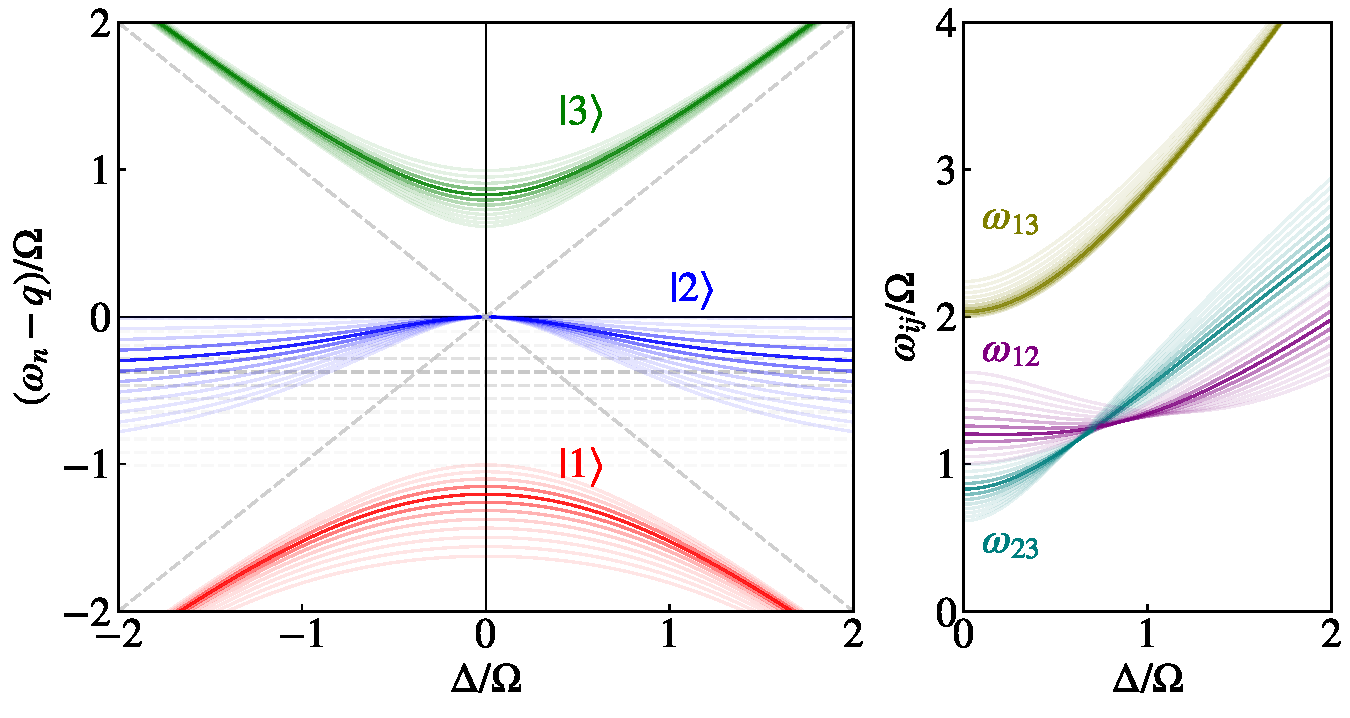
\includegraphics[width=\columnwidth]{figure_1.pdf}
    \caption{
    \label{fig:eigensystem_schematic}
        Energy spectrum and splittings of a radiofrequency coupled spin-1 for various $q_R = q/\Omega \in [0,1]$.
        The transparency of each curve is proportional to the distance of $q_R$ from $\qRmagic$ in \refeq{eq:qRmagic}.
        (Left) Energies $\omega_n$ of dressed states $\ket{n}=\ket{1}$, (red) $\ket{2}$ (blue), and $\ket{3}$ (green) normalized to the Rabi frequency $\Omega$ as a function of detuning $\Delta$,
        Dashed lines indicate the energies of uncoupled states ($\Omega=0$) in a frame rotating at $\omega_{\text{rf}}$.
        (Right) Splittings $\omega_{ij} = \omega_j - \omega_i$ of dressed states $\ket{i}$ and $\ket{j}$ as a function of detuning.
        When $q_R=\qRmagic$ (bold curves), energies $\omega_1$ and $\omega_2$ share the same curvature, and their difference $\omega_{12}$ is minimally sensitive to detuning and thus magnetic field variations.
    }
\end{figure}
This yields dressed eigenstates $\{\ket{1}, \ket{2}, \ket{3}\}$ that are no longer $\text{SO}(3)$ rotations of the bare Zeeman states $\ket{m_z}$, and an eigenspectrum $\omega_i(\Delta) = E_{\ket{i}}/\hbar$ shown in \reffig{fig:eigensystem_schematic} (left).
% ($\expect{\vect{\hat{F}}^2} < \hbar^2$)

Moreover, the couplings between these dressed states when $q \neq 0$ are markedly different:
$\bra{1} \hat{F}_{y,z} \ket{2}$ and $\bra{2} \hat{F}_{y,z} \ket{3}$ remain non-vanishing but $\bra{1} \hat{F}_x \ket{3}$ becomes non-zero.
The transitions are thus cyclic ($\ket{1} \leftrightarrow \ket{2} \leftrightarrow \ket{3} \leftrightarrow \ket{1}$) and non-degenerate, characterized by a dressed Larmor frequency $\omega_D\equiv(\omega_3-\omega_1)/2$, and dressed quadratic shift $q_D \equiv (\omega_3 + \omega_1 -2\omega_2)/2$, giving splittings $\omega_{23}=\omega_D-q_D$, $\omega_{12}=\omega_D+q_D$ and $\omega_{13}=2\omega_D$.
On resonance, $\omega_D=\sqrt{\Omega^2+q_D^2}$ and $q_D = -q/2$.

A figure-of-merit for decoupling is the curvature of the transition frequency at resonance.
In a dressed two-level system there is one convex and one concave eigenstate whose splitting is simply convex.
Figure 1 shows that in the spin-1 system with quadratic shift, two states are convex.
This suggests that a regime may exist in which the curvature of their transition frequency vanishes~\cite{rabl_strong_2009,*xu_coherence-protected_2012}.
Indeed we find an analytic value of the normalized quadratic shift $q_R=q/\Omega$ where the curvatures of $\omega_1$ and $\omega_2$ are equal~\footnote{
  The curvature of the dressed-state energies is evaluated using perturbation theory. In particular, the dimensionless curvature of $\omega_{12}$ is $\partial^2(\omega_{12}/\Omega)/\partial(\Delta/\Omega)^2 = \Omega \, \partial^2\omega_{12}/\partial \Delta^2 = -(3 q_R \sqrt{4 + q_R^2} - q_R^2 - 2)/\sqrt{4 + q_R^2}$. For $q_R = 0$, we recover the spin-1/2 result, $\Omega\, \partial^2\omega_{12}/\partial \Delta^2 = 1$.},
\begin{align}
\label{eq:qRmagic}
    \qRmagic = \sqrt{(3\sqrt{2} - 4)/2} \approx 0.348 \, ,
\end{align}
resulting in the vanishing quadratic dependence of the transition frequency $\omega_{12}=\omega_2 - \omega_1$ on $\Delta$.
% A similar regime was identified in a multiply-dressed three-level $V$-system~\cite{rabl_strong_2009,*xu_coherence-protected_2012}.
The leading-order sensitivity of these states to field variations $\delta B_z$ at $\qRmagic$ is quartic~\footnote{
    We take $\Delta = -\gamma \, \delta B_z$ for $|\Delta | \leq 2\Omega$ ($| \delta B_z | \leq B_{\text{rf}}/2$) and $| \partial q / \partial \Delta | \approx | \gamma^{-1} \partial q / \partial B_z | = |2 B_z q_Z / \gamma| \ll 1$, valid to $10^{-3}$ for the field strengths $B_z \lesssim \unit[5]{G}$ used here, resulting in vanishing third-order derivatives of $\omega_i$ with respect to detuning. 
    In general, the variation of $q$ with $\Delta$ (or $\delta B_z$) can be accounted for using the Breit-Rabi equation, leading to a residual linear and cubic variation of $\omega_{12}$ with $\delta B_z$, and a small correction to $\qRmagic$ in \refeq{eq:qRmagic}.},
giving the subspace comprised of ${\ket{1},\ket{2}}$ a higher-order decoupling than can be achieved with a two-level system; we join Dimitris~\etal in terming these `synthetic clock states'.

We explore this high-order decoupling in the laboratory with a continuous measurement of the dressed spectrum of a spin-1 non-degenerate quantum gas.
Using a single realization of the quantum gas we make many successive weak measurements, revealing all three splittings $\omega_{ij}$ simultaneously.
Our spinor quantum gas apparatus~\cite{wood_magnetic_2015} and Faraday atom-light interface~\cite{jasperse_magic-wavelength_2017} are described elsewhere.
We prepare an ultracold gas ($\sim \unit[1]{\upmu K}$) of approximately $10^6$ \Rb atoms in a crossed-beam optical dipole trap.
A radiofrequency field of amplitude $\Omega/2\pi \leq \unit[100]{kHz}$ couples the three Zeeman states $\ket{m_z=-1,0,+1}$ of the lowest hyperfine ground state.
To perform a weak measurement of the evolving spin, we focus onto the atoms a linearly polarized far-off-resonant probe beam ($\lambda=\unit[781.15]{nm}$, red detuned $\unit[0.45]{THz}$) propagating along $x$.
The spin component parallel to the wavevector of the probe rotates its polarization via the paramagnetic Faraday effect; shot-noise limited polarimetry measures $\expect{\hat{F}_x}$ as an modulated tone near $\omega_L$.
Similar weak continuous Faraday measurements have tracked spin-mixing dynamics of a polar spinor condensate~\cite{liu_quantum_2009} and enabled quantum state tomography~\cite{smith_continuous_2004,smith_efficient_2006}.

To probe the dressed state spectrum and coherences, we prepare a superposition of dressed states by suddenly turning on the Rabi coupling $\Omega$, projecting the polarized collective spin $\ket{m_z=-1}$ onto $\ket{\psi(t=0)} = \sum_i c_i \ket{i}$.
The total magnetic field in the laboratory frame is $\vect{B}(t \geq 0) = -B_{\text{rf}} \cos (\omega_{\text{rf}} t) \vect{e}_x + B_z(t) \vect{e}_z$, where $B_z(t)$ varies slowly compared to $\Omega$.
The resulting Faraday signal is analyzed in the time-frequency domain using the short-time Fourier transform (STFT), revealing the rich frequency and amplitude modulation related to the dressed state energies, coherences, and coupling strengths.

With no deliberate variation of the Rabi frequency or detuning, we observe the STFT amplitude (spectrogram) shown in \reffig{fig:static_coupling}.
Strong amplitude modulation of the Faraday signal is apparent as three pairs of sidebands, each equidistant from the carrier frequency $f_{\text{rf}} = \omega_{\text{rf}}/2\pi$. 
\begin{figure}
    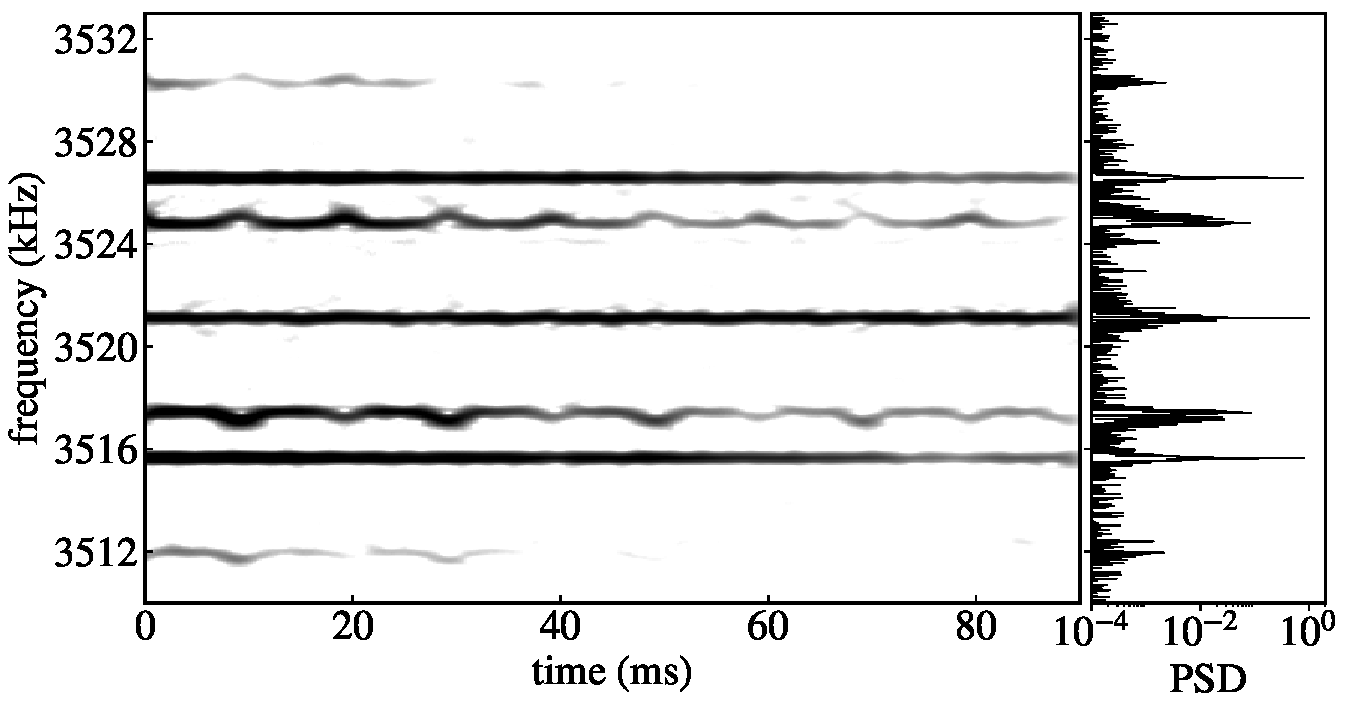
\includegraphics[width=\columnwidth]{figure_2.pdf}
    \caption{
    \label{fig:static_coupling}
    Continuous measurement of the dressed energy spectrum for $q_R = 0.402(3)$, $f_{\text{rf}}=\unit[3.521]{MHz}$ and $B_0=\unit[5.013]{G}$ (left) and the power spectral density (PSD, normalized) of the $\unit[90]{ms}$ long signal (right). 
    (Inset) The dressed state energy diagram for resonant coupling ($\abs{\Delta} \ll \Omega$); the mean and difference of transition frequencies $\omega_{12}$ and $\omega_{23}$ is the dressed Larmor frequency $\omega_D$ and quadratic shift $q_D$, respectively.
    The upper sidebands about the carrier at $f_{\text{rf}}$ are associated with the $\omega_{13}$ (gold), $\omega_{23}$ (turquoise), and $\omega_{12}$ (lavender) transitions.
    % Magnetic field fluctuations induced by mains power are manifest as asymmetric frequency modulation of the $\omega_{13}$ and $\omega_{23}$ sidebands, while the $\omega_{12}$ transition remains relatively unaffected.
    The corresponding spectral peaks have linewidths $\unit[102]{Hz}$, $\unit[97]{Hz}$, and $\unit[24]{Hz}$, respectively.
    The $\omega_{12}$ linewidth is near transform-limited, whereas the broadened peaks of the less decoupled $\omega_{23}$ transition exhibit a skew (third-moment) of $\unit[84]{Hz}$ (upper sideband) and $-\unit[100]{Hz}$ (lower sideband).
    }
\end{figure}
Each pair of sidebands corresponds to a dressed state transition $\ket{i} \leftrightarrow \ket{j}$; with sideband frequencies  $f_{\text{rf}} \pm f_{ij}$ where $f_{ij} = \omega_{ij}/2\pi$.
Thus the spectrogram is a calibration-free, real-time measurement of the dressed state spectrum.
Restricting attention to the upper sidebands, the two closest to the carrier are from adjacent state transitions $\omega_{12}$ and $\omega_{23}$ with similar amplitudes and at frequencies $\omega_D \pm q_D$ above the carrier.
The third, weaker sideband $2\omega_D$ above the carrier signifies the cyclic $\ket{1} \leftrightarrow \ket{3}$ transition, appearing when $q\neq 0$. 
No attempt was made to shield the apparatus from magnetic noise.
The power line causes a temporally varying $\delta B_z = \delta B_{\text{line}}(t)$ at the line frequency of $\unit[50]{Hz}$ and its odd harmonics, of $\unit[1.4]{mG}$ ($\unit[1]{kHz}$) peak-to-peak amplitude.
Each dressed transition is affected by the magnetic fluctuations differently: the sidebands corresponding to the $\omega_{13}$ and $\omega_{23}$ transitions exhibit asymmetric frequency modulation, whereas the optimally decoupled $\omega_{12}$ transition remains unperturbed within the frequency resolution of this spectrogram.
The normalized power spectral density (\reffig{fig:static_coupling}, right) of the entire time-series yields maximum frequency resolution at the expense of all temporal resolution.
The $\omega_{12}$ transition is unskewed and has a near transform-limited width, four times narrower than the outwardly-skewed $\omega_{23}$ and $\omega_{13}$ sidebands. We quantify the skew using the Pearson skew coefficient which is significant for the $\omega_{23}$ band with an average of 0.875, 11 times larger than the $\omega_{12}$ band coefficient of 0.08. 
\begin{figure}
    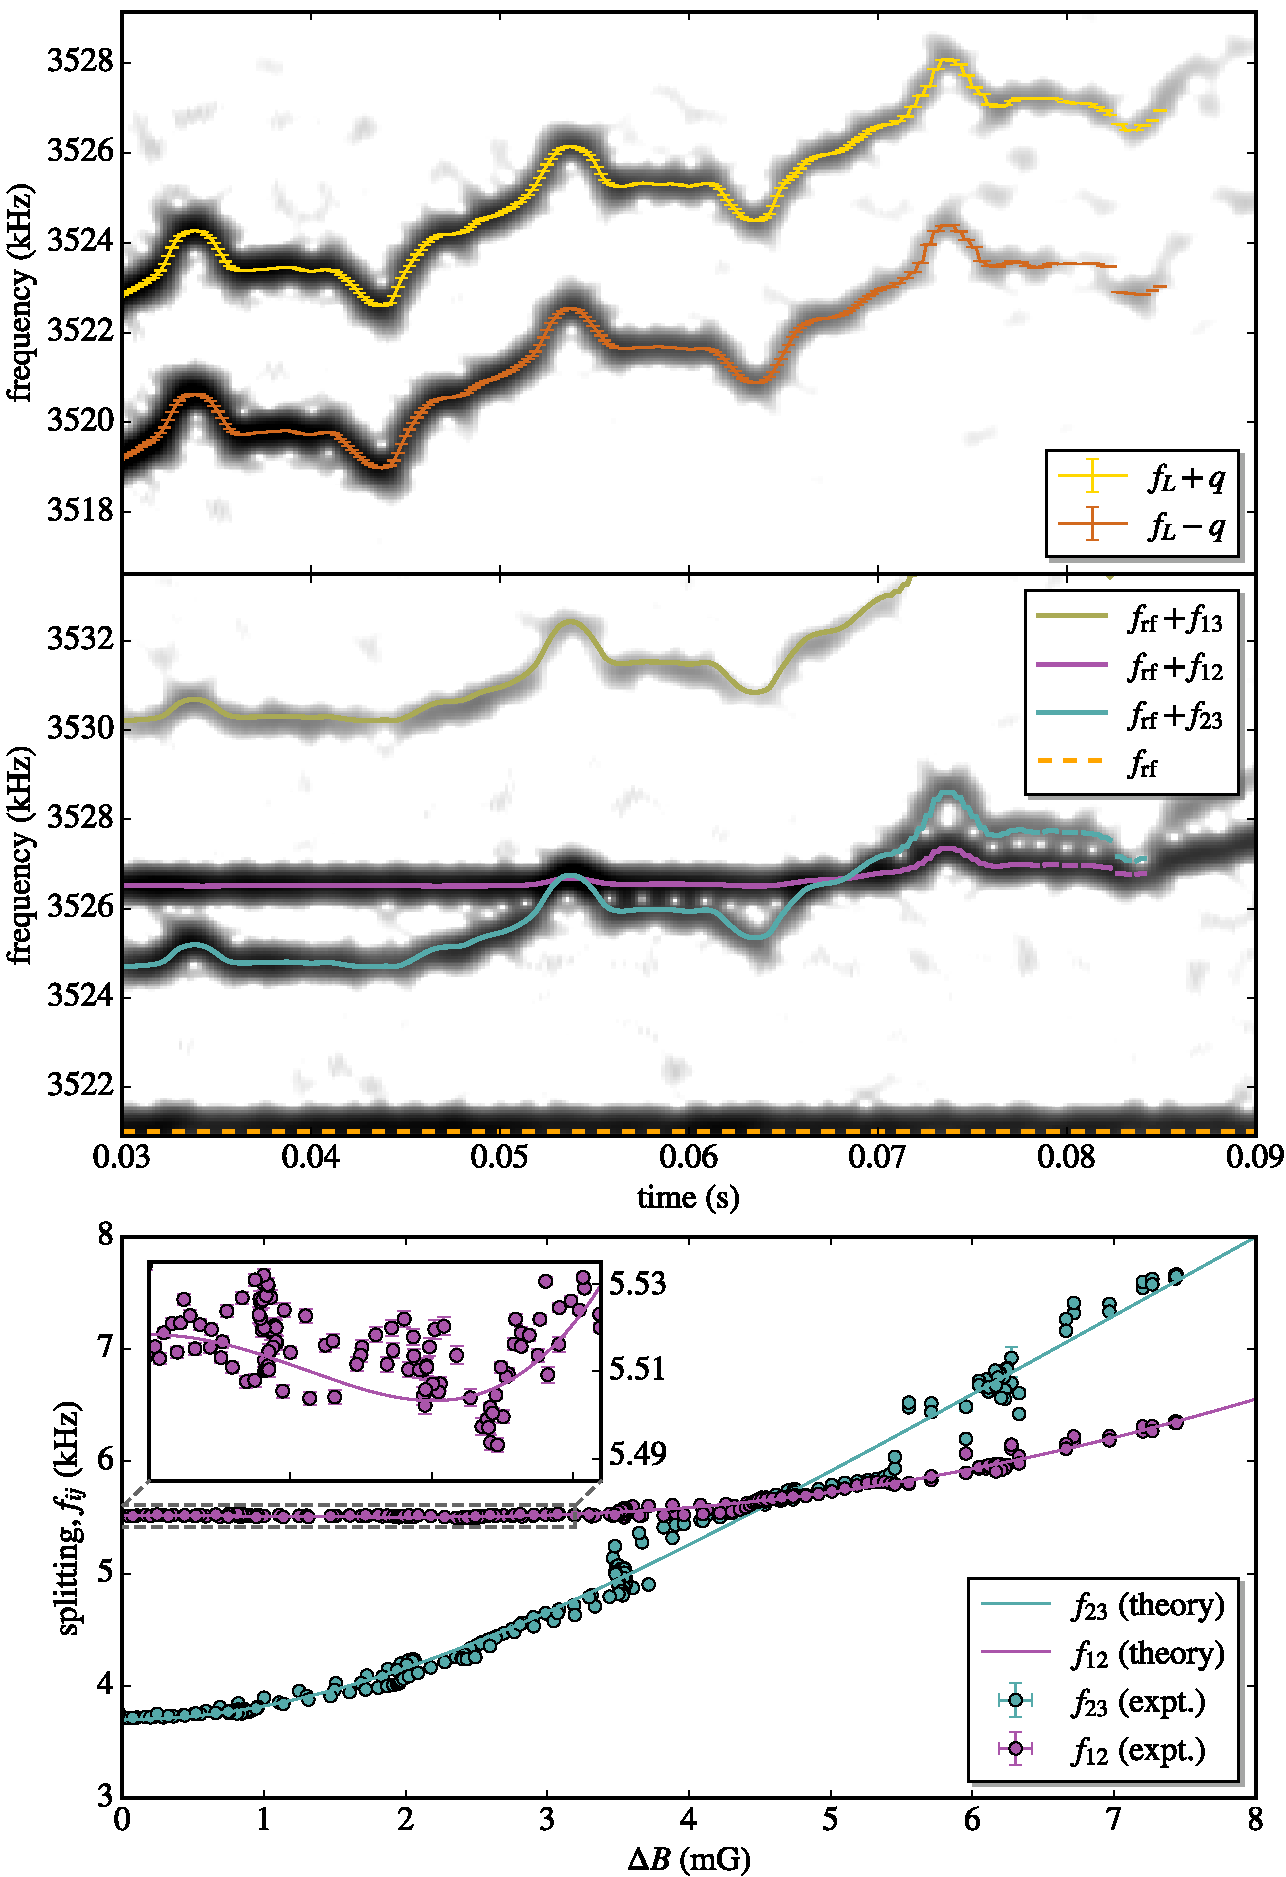
\includegraphics[width=\columnwidth]{figure_3.pdf}
    \caption{
    \label{fig:acquisition_pipeline}
        Real-time observation of continuous dynamical decoupling for $q_R = 0.402(3)$.
        (a) and (b) are spectrograms of a continuous weak measurement of $\expect{\hat{F}_x}$.
        (a) Magnetometry of the bare Zeeman states ($\Omega=0$) is used to calibrate $B_z(t) = B_0 + \delta B_z(t)$ during the measurement interval, in which the field [detuning] varies over a range $\sim B_{\text{rf}}$ [$2\Omega$].
        We numerically track the Zeeman splittings (gold/orange) to determine the instantaneous Larmor frequency $\omega_L(t)$ and quadratic shift $q(t)$.
       (b) The field is swept over the same range but the rf dressing is applied ($\Omega/2\pi = \unit[4.520(2)]{kHz}$).
       Three sidebands above (shown) and below the carrier at $f_{\text{rf}}=\unit[3.521]{MHz}$ (dashed, orange) reveal the dressed state splittings $f_{ij} = \omega_{ij}/2\pi$.
       (c) A parametric plot of $f_{12}(t)$ and $f_{23}(t)$ versus $\delta B_z(t)$ by combining analysis of (a) and (b).
       Solid curves in (b) and (c) are theoretical splittings from an eigenspectrum calculation, provided only $f_{\text{rf}}$, $B_z(t)$, and $\Omega$, i.e. no free parameters.
       Variation of the synthetic clock transition $f_{12}$ for $0 \leq \delta B_z \leq B_{\text{rf}}/4 = \unit[3.2]{mG}$ (c, inset).
    }
\end{figure}

The amplitude of each sideband is proportional to the corresponding dressed-state coherence $\rho_{ij} = c_i^* c_j $, and the non-vanishing dressed state coupling(s) $\bra{i} \hat{F}_{x,y,z} \ket{j}$.
\begin{table*}[t]
    \caption{Upper sidebands of the Faraday rotation signal $\propto \expect{\hat{F}_x}$ of an arbitrary dressed state superposition.
    Each sideband is identified with a dressed-state transition $\ket{i} \leftrightarrow \ket{j}$.
    Sideband frequencies are reported in both absolute terms and relative to the carrier at $\omega_{\text{rf}}$.
    Sideband amplitudes are for resonant coupling ($\Delta = 0$), and
    for the initial state $\ket{\psi(t=0)}=\ket{m_z=-1}$ these can be concisely expressed in terms of the dressed Larmor frequency $\omega_D$ and quadratic shift $q_D$.
    For each upper sideband, there is a lower sideband of the same amplitude, relative frequency, and opposite phase.
    \label{tab:sidebands}
    }
    \begin{ruledtabular}
    \begin{tabular}{ccccc}
    transition & frequency & $\omega_{ij} - \omega_{\text{rf}}$ & amplitude ($\Delta = 0$) & amplitude ($\Delta = 0$, $\ket{m_z=-1}$) \\ \hline
     (carrier) & $\omega_{\text{rf}}$ & 0 & $(\bra{3} \hat{F}_x \ket{3} - \bra{1} \hat{F}_x \ket{1}) (\rho_{33} - \rho_{11})$  & $\hbar q_D \Omega/2 \omega_D^2$ \\
     $\ket{1} \leftrightarrow \ket{2}$ & $\omega_{\text{rf}} + \omega_{12}$ & $\omega_D+q_D$ & $-2i \bra{1} \hat{F}_y \ket{2} \text{Re}\,\rho_{12} = -2 \bra{2} \hat{F}_z \ket{3} \text{Re}\,\rho_{12}$ & $\hbar \Omega/4 \omega_D$ \\
     $\ket{2} \leftrightarrow \ket{3}$ & $\omega_{\text{rf}} + \omega_{23}$ & $\omega_D-q_D$ & $2i \bra{2} \hat{F}_y \ket{3} \text{Re}\,\rho_{23} = 2 \bra{1} \hat{F}_z \ket{2} \text{Re}\,\rho_{23}$ & $\hbar \Omega/4 \omega_D$ \\
     $\ket{1} \leftrightarrow \ket{3}$ & $\omega_{\text{rf}} + \omega_{13}$ & $2\omega_D$ & $2 \bra{1} \hat{F}_x \ket{3} \text{Re}\,\rho_{13}$ & $\hbar q_D \Omega/4 \omega_D^2$
    \end{tabular}
    \end{ruledtabular}
\end{table*}
Analytic expressions for the sideband amplitudes near resonance ($\abs{\Delta} \ll \Omega$) are summarized in Table~\ref{tab:sidebands}.
If the projection onto the dressed basis (and hence $\rho_{ij}$) is known, our measurement constitutes a single-shot estimation of the coupling strengths.  
Alternatively, if the couplings are separately characterized~\cite{dimitris_synthetic_2017}, this amounts to continuous measurement of the dressed density matrix, effecting quantum state estimation of the dressed system.

Different platforms use different metrics for the fidelity of dynamical decoupling, and in addition to linewidth narrowing include prolonged coherence.
We observe a three-fold increase in the lifetime of the spectral components corresponding to the $\omega_{12}$ and $\omega_{23}$ transitions as compared with the undressed system (\reffig{fig:acquisition_pipeline}a, $1/e$ decay time \unit[23.8(2)]{ms}).
Dressed-state coherences are expected to last longer, but were limited here by the $\sim\unit[100]{ms}$ probe-induced photon scattering time.
A less perturbative probe~\cite{jasperse_magic-wavelength_2017} should reveal even longer dressed coherence times at the expense of signal-to-noise ratio. 

To better expose the enhanced decoupling of the synthetic clock states in the vicinity of $\qRmagic$, we swept the the magnetic field over a wider range than was furnished by the power line noise.
The longitudinal field $B_z(t) = B_0 + \alpha t + B_{\text{line}}(t)$, where $\alpha = \unit[128]{mG/s}$ is the linear sweep rate; the resulting detuning sweeps across $2\Omega$ (\textit{cf.} the domain of~\reffig{fig:eigensystem_schematic}) during the single-shot measurement.
We interleave each dressed state realization (or `shot') of the experiment with a magnetometry shot calibrating $B_z(t)$: an rf $\pi/2$-pulse initiates Larmor precession of the undressed collective spin, and the Faraday signal is composed of two tones at $\omega_\pm = \omega_L \pm q$, the Zeeman splittings (\reffig{fig:acquisition_pipeline}, top).
For $q \, \tau_f \geq 2\pi$, where $\tau_f$ is the length of the spectrogram window, $\omega_\pm$ are resolved yielding the instantaneous $\omega_L(t)$ and $q(t)$.
We then use $\omega_L(t)$ to find $\delta B_z(t)$ (and $\Delta(t)$) by inverting the Breit-Rabi equation~\cite{ramsey_molecular_1956}~\footnote{
    The experiment is synchronized to the mains power line; the harmonic composition varies little between successive shots ($\unit[20]{s}$ apart), and thus the calibration $\delta B_z(t)$ and $q(t)$ are good proxies for the values experienced by the atoms in the subsequent decoupled shot.
}.

We measured the dressed spectrum for resonant magnetic fields $B_0$ ranging from $3.549$ to $\unit[5.568]{G}$ (applied rf frequencies $f_{\text{rf}}$ from $2.493$ to $\unit[3.911]{MHz}$), with a mean Rabi frequency of $\Omega/2\pi = \unit[4.505(3)]{kHz}$ ($B_{\text{rf}} = \unit[12.83(1)]{mG}$).
At each field $B_0$ we ensured the Rabi frequency was fixed by measuring the voltage drop across the coil at $f_{\text{rf}}$ with an rf lock-in amplifier.
The Rabi frequency was ultimately measured using the atoms by analyzing the dressed energy spectrum near resonance ($\abs{\Delta}/2\pi \leq \unit[100]{Hz}$) where $\Omega = \sqrt{\omega_{12} \omega_{23}}$.
The measured Rabi frequencies had a standard deviation $\sigma(\Omega)/2\pi = \unit[9.4]{Hz}$, validating the above method.

Figure~\ref{fig:acquisition_pipeline} shows the dressed spectrum measured as $\delta B_z$ varies across a range $\sim B_{\text{rf}}$ during a single-shot.
The instantaneous dressed state splittings for all three transitions were predicted with no free parameters, and are plotted atop the spectrogram data, showing excellent agreement with the measured sidebands.
Line noise renders $\delta B_z(t)$ neither linear nor monotonic.
By tracking the instantaneous peaks in the calibration and dressed spectrograms we plot $(\delta B_z(t), f_{ij}(t))$ parametrically, eliminating the line noise systematic.
The sensitivity of the $\ket{1} \leftrightarrow \ket{2}$ and $\ket{2} \leftrightarrow \ket{3}$ transitions to magnetic field variations is shown in \reffig{fig:acquisition_pipeline}c.
The synthetic clock transition is most insensitive; $f_{12}$ varies by $\unit[39]{Hz}$ (expt.), $\unit[26]{Hz}$ (theory) for $0 \leq \delta B_z \leq B_{\text{rf}}/4 = \unit[3.2]{mG}$ (\reffig{fig:acquisition_pipeline}c, inset).
Normalizing the variation to the Rabi frequency makes possible a comparison of the decoupling across platforms and ac magnetometry bandwidths. 
The normalized variation $\omega_{12}/\Omega = 8.6\times10^{-3}$ (expt.) and $5.8\times10^{-3}$ (theory) across a detuning range of half a Rabi frequency.
By comparison, the normalized variation for conventional decoupling ($q_R=0$) is $(\sqrt{5}-2)/2 \approx 0.118$; 14 (expt.) and 20 (theory) times higher than the variation.
Alternatively, the normalized variation of the $\ket{m_z=\pm1} \leftrightarrow \ket{m_z = 0}$ Zeeman transitions in the low-field limit is $0.5$; 58 (expt.) and 86 (theory) times higher than the variation in the synthetic clock transition frequency.

\begin{figure}
    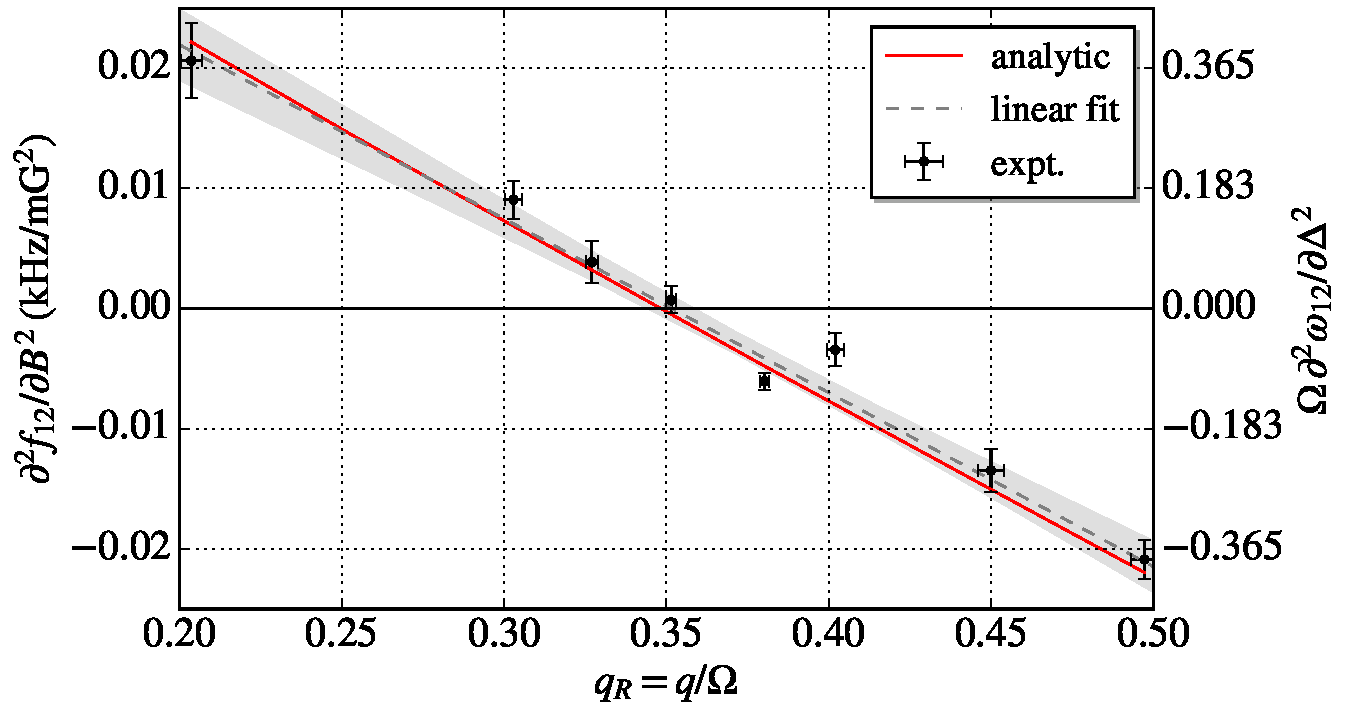
\includegraphics[width=\columnwidth]{figure_4.pdf}
    \caption{
    \label{fig:curvature_vs_qR}
        Curvature of the synthetic clock transition for relative quadratic shifts $q_R \in [0.2, 0.5]$.
        The measured curvature (black points) was determined from polynomial fitting to $(\delta B_z, f_{12})$ data, e.g. \reffig{fig:acquisition_pipeline}(c).
        Vertical and horizontal error bars correspond to the standard error of the regression and uncertainty in $q_R$ (via $u(q)$ and $u(\Omega)$ at each field $B_0$), respectively.
        A linear fit (black, dashed) with 1$\sigma$ confidence band (gray, shaded) are shown, whose intercept can be used to impute $\qRmagic\text{ (expt.)} = 0.350(6)$.
        The analytic expression for the curvature (red)~\cite{Note1} is consistent with the data-driven analysis of the curvature, \textit{cf.} $\qRmagic\text{ (theory)} = 0.348$.
        The left [right] vertical axis shows the curvature $\partial^2 f_{12}/\partial B_z^2$ [$\Omega\, \partial^2\omega_{12}/\partial \Delta^2$] in absolute units of $\unit{kHz/G^2}$ [dimensionless units].
        The normalized curvature is unity when $q_R=0$.
    }
\end{figure}
 
To optimally suppress the sensitivity of the synthetic clock states to small field variations, we experimentally determined the curvature of $\omega_{12}$  for $q_R$ between 0.2 and 0.5, independent of the predicted spectrum of $\ham_{\text{rwa}}$.
For each $q_R$, we fit a polynomial to $(\delta B_z, f_{12})$ data to extract $\partial^2 f_{12}/\partial B_z^2$ (\reffig{fig:curvature_vs_qR}).
The predictive power of the measured dressed spectrum and this model-independent analysis is affirmed by the agreement with the theoretical curvature.
We perform linear~\note{LDT: explain why!} regression of the measured curvature versus $q_R$ to infer $\qRmagic\text{ (expt.)} = 0.350(6)$, in agreement with the theoretical value in~\refeq{eq:qRmagic}.
The lowest curvature we measured was $\left(\partial^2 f_{12}/\partial B_z^2\right)_{\text{min}} = \unit[0.7]{Hz/mG^2}$ at $q_R = 0.351(2)$.
In dimensionless units -- with the splitting and detuning normalized to the Rabi frequency -- $\left(\Omega\, \partial^2\omega_{12}/\partial \Delta^2\right)_{\text{min}} = 0.013$, $\sim 75$ times lower than the curvature of this transition for quadratic decoupling ($q_R = 0$).

This intra-shot revelation of the time and frequency domain renders the measurement of these spectra orders of magnitude more efficient.
For example, the single spectrum shown in \reffig{fig:acquisition_pipeline} would take $\sim (10$ shots per $\delta B_z$ per $\omega_{ij} ) \times (20$ distinct $\delta B_z$) $\times (3 $ transitions $\omega_{ij}) = 600$ shots, or $\sim \unit[1.2\times10^4]{s} = 200$ minutes of data acquisition.
We acquire this spectrum in a single shot, i.e. $\unit[20]{s}$.
The data used to generate \reffig{fig:curvature_vs_qR} was acquired in only $5$ minutes.

In summary, we have demonstrated contiuous measurement of continuous dynamical decoupling in a spin-1 quantum gas.
%and expeditious optimization of this decoupling by varying the the relative asymmetry of the Zeeman state splittings.
Continuous weak measurement via the Faraday effect yields information about the rf-dressed superposition, the dressed-state couplings and energies, simultaneously, making possible full characterisation over detunings in a single experimental shot. 
The cyclic coupling we observe is a sought-after for emaulation of quantum spin ladders with frustrated interactions~\cite{??}.
The phase space of spin-orbit coupled spin-1 Bose gases 
the coupling spatially dependent, the optimal decoupling of the synthetic clock states demonstrated can be applied to , as $q = \qRmagic \Omega$ traverses the polar-striped and plane-wave phases in the vicinity of a tricritical point of the $(\Omega, q)$ phase diagram~\cite{martone_tricriticalities_2016}.
% Remove: negative
In this measurement regime, we do not resolve the quantum noise of the decoupled collective spin.
With a modification of the probe (atom-shot noise dominated) we could measure and affect the quantum noise dynamically,
and probing the dressed state coherences in this regime may expose non-Gaussian quantum noise geometries in a manner analogous to Ref.~\cite{colangelo_simultaneous_2017}.
Our time-frequency reduction of the weak measurement record makes plain the cyclic coupling of all three dressed states, which could be applied to emulating quantum spin ladders with frustrated interactions~\cite{??}.

Indeed the Faraday probe beam -- used to detect magnetization -- could constitute one of the Raman beams used to generate the spin-orbit coupling.

We thank A. A. Wood, N. Lundblad, I. B. Spielman, and F. A. Pollock for useful conversations. This work was supported by ARC LP130100857. 

\bibliography{dressed_faraday}

\end{document}
        
